\documentclass[a4paper,12pt]{article}
\usepackage{amsmath,amssymb,amstext,graphicx}

\title{Der Test}
\author{Ich}
\date{\today{}, Potsdam}

\usepackage[automark]{scrpage2}
\pagestyle{scrheadings}
\clearscrheadfoot
\ifoot[]{\author}
\ofoot[]{\pagemark} 

\begin{document}
\maketitle 
\newpage 
\tableofcontents
\newpage
\begin{flushright}
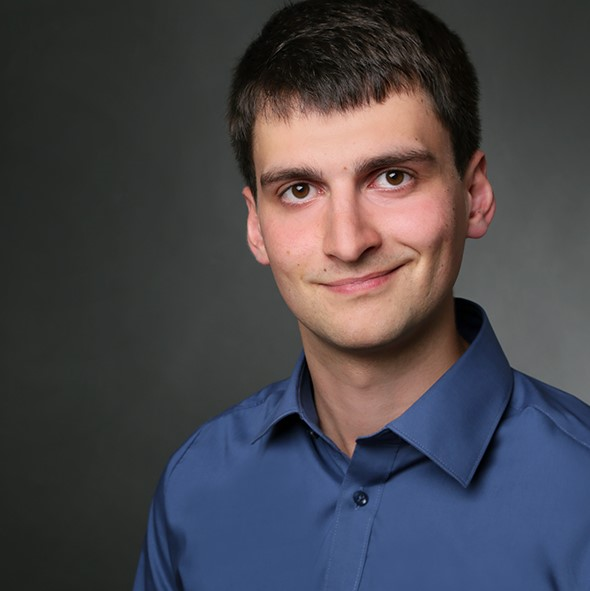
\includegraphics[scale=0.2]{Kemter} 
\end{flushright}



\section{Section}
\label{sec:Ober}
\subsection{Subsection1}
\label{sec:Unter1}

\begin{center}
	\begin{equation}
  	\label{eq:squareroot}
  	c = \sqrt{ a^{2} + b^{2} }
	\end{equation}
\end{center}



\begin{enumerate}
\item Kram
\item Zeug
	\begin{itemize}
	\item Unterzeug
	\item Mehr Unterzeug
	\end{itemize}
\end{enumerate}

\subsection{Subsection2}
\label{sec:Unter2}
Im Abschnitt \ref{sec:Unter1} auf Seite \pageref{sec:Unter1} habe ich
gezeigt dass \eqref{eq:squareroot} der allgemeinen...

\end{document}